
\documentclass[11pt]{article}

% Paquetes
%===================================================================================================

% Establecemos los márgenes
\usepackage[a4paper, margin=1in]{geometry}

% Separacion entre parrafos
\setlength{\parskip}{1em}

% Paquete para incluir codigo
\usepackage{listings}

% Paquete para incluir imagenes
\usepackage{graphicx}
\graphicspath{ {./images/} }

% Para fijar las imagenes en la posicion deseada
\usepackage{float}

% Para que el codigo acepte caracteres en utf8
\lstset{literate=
  {á}{{\'a}}1 {é}{{\'e}}1 {í}{{\'i}}1 {ó}{{\'o}}1 {ú}{{\'u}}1
  {Á}{{\'A}}1 {É}{{\'E}}1 {Í}{{\'I}}1 {Ó}{{\'O}}1 {Ú}{{\'U}}1
  {à}{{\`a}}1 {è}{{\`e}}1 {ì}{{\`i}}1 {ò}{{\`o}}1 {ù}{{\`u}}1
  {À}{{\`A}}1 {È}{{\'E}}1 {Ì}{{\`I}}1 {Ò}{{\`O}}1 {Ù}{{\`U}}1
  {ä}{{\"a}}1 {ë}{{\"e}}1 {ï}{{\"i}}1 {ö}{{\"o}}1 {ü}{{\"u}}1
  {Ä}{{\"A}}1 {Ë}{{\"E}}1 {Ï}{{\"I}}1 {Ö}{{\"O}}1 {Ü}{{\"U}}1
  {â}{{\^a}}1 {ê}{{\^e}}1 {î}{{\^i}}1 {ô}{{\^o}}1 {û}{{\^u}}1
  {Â}{{\^A}}1 {Ê}{{\^E}}1 {Î}{{\^I}}1 {Ô}{{\^O}}1 {Û}{{\^U}}1
  {ã}{{\~a}}1 {ẽ}{{\~e}}1 {ĩ}{{\~i}}1 {õ}{{\~o}}1 {ũ}{{\~u}}1
  {Ã}{{\~A}}1 {Ẽ}{{\~E}}1 {Ĩ}{{\~I}}1 {Õ}{{\~O}}1 {Ũ}{{\~U}}1
  {œ}{{\oe}}1 {Œ}{{\OE}}1 {æ}{{\ae}}1 {Æ}{{\AE}}1 {ß}{{\ss}}1
  {ű}{{\H{u}}}1 {Ű}{{\H{U}}}1 {ő}{{\H{o}}}1 {Ő}{{\H{O}}}1
  {ç}{{\c c}}1 {Ç}{{\c C}}1 {ø}{{\o}}1 {å}{{\r a}}1 {Å}{{\r A}}1
  {€}{{\euro}}1 {£}{{\pounds}}1 {«}{{\guillemotleft}}1
  {»}{{\guillemotright}}1 {ñ}{{\~n}}1 {Ñ}{{\~N}}1 {¿}{{?`}}1 {¡}{{!`}}1
}

% Para que no se salgan las lineas de codigo
% Para fijar una fuente que resalte
\lstset{breaklines=true, basicstyle=\ttfamily}

% Para que los metadatos que escribe latex esten en español
\usepackage[spanish]{babel}
\decimalpoint % Para que no se cambie el punto a la coma

% Para la bibliografia
% Sin esto, los enlaces de la bibliografia dan un error de compilacion
\usepackage{url}

% Para que se puedan clicar los enlaces
\usepackage{hyperref}

% Para mostrar graficas de dos imagenes, cada una con su caption, y con un caption comun
\usepackage{subcaption}

% Simbolo de los numeros reales
\usepackage{amssymb}

% Para que los codigos tengan una fuente distinta
\usepackage{courier}

\lstdefinestyle{CustomStyle}{
  language=Python,
  numbers=left,
  stepnumber=1,
  numbersep=10pt,
  tabsize=4,
  showspaces=false,
  showstringspaces=false
  basicstyle=\tiny\ttfamily,
}

% Para referenciar secciones usando el nombre de las secciones
\usepackage{nameref}

% Para enumerados dentro de enumerados
\usepackage{enumitem}

% Para mejores tablas
\usepackage{tabularx}

% Para poder tener el mismo identificador en dos tablas separadas
\usepackage{caption}

% Mostrar la página de las referencias en el indice del documento
\usepackage[nottoc,numbib]{tocbibind}

% Para mostrar las matrices
\usepackage{amsmath}

% Para que las notas al pie de pagina queden bien abajo
\usepackage[bottom]{footmisc}

% Para poner tablas en horizontal, ocupando bien la página
% cuando hay mucho texto en la table
\usepackage{lscape}

% Comandos personalizados
%===================================================================================================
% Here all custom commands are defined

% Para realizar las citas de forma corta
\newcommand{\customcite}[1]{\emph{"\ref{#1}. \nameref{#1}"}}

% Para entrecomillar un texto
\newcommand{\entrecomillado}[1]{\emph{``#1''}}




% Metadatos del documento
%===================================================================================================
\title{
    Estudio sobre la empleabilidad de los estudiantes
}

\author{
    {Sergio Quijano Rey}\\
    {sergioquijano@correo.ugr.es}
}

\date{\today}

% Separacion entre parrafos
\setlength{\parskip}{1em}

% Contenido del documento
%===================================================================================================
\begin{document}

% Portada del documento
\maketitle
\pagebreak

% Indice de contenidos
\tableofcontents

% Lista de figuras
% Uso el addtocontents para que no se muestre la seccion de indice de figuras en el indice inicial

\addtocontents{toc}{\setcounter{tocdepth}{-10}}
\listoffigures

\listoftables

% \lstlistoflistings
\addtocontents{toc}{\setcounter{tocdepth}{3}}

\pagebreak

% Contents of the document

\section{Abstract}

En este trabajo, estudiaremos una base de datos consistente en métricas recogidas durante entrevistas de prueba, junto a si los candidatos son o no escogidos para el hipotético puesto de trabajo.

Con \textbf{dos objetivos} en mente:

\begin{itemize}
    \item Construir un clasificador eficiente para predecir la empleabilidad
    \item Usar la base de datos para realizar un estudio sobre lo meritocrático del proceso. Dicho experimento consiste en entrenar dos modelos, uno usando las variables que consideramos meritocráticas, y otro usando las variables que consideramos no meritocráticas. Si el modelo que usa variables no meritocráticas funciona mejor, podemos pensar que entonces el proceso de selección se basa más en estos aspectos, que hemos considerado no meritocráticos
\end{itemize}

Para ello, realizaremos:

\begin{itemize}
    \item Un estudio univariante de la base de datos, destacando el tratamiento de \textit{outliers}, el estudio de la normalidad univariante, y un análisis descriptivo clásico
    \item Un estudio multivariante de la base de datos, destacando el estudio de las correlaciones entre variables, tratamiento multivariante de \textit{outliers}, estudio de normalidad multivariante y reducción de la dimensionalidad con \textit{PCA} y \textit{FA}
    \item Ajuste de los modelos, destacando una pequeña exploración de hiperparámetros, entrenamiento y validación, comparando los resultados
    \item El experimento adicional, previamente mencionado
\end{itemize}

Al final, conseguimos obtener un modelo muy robusto a la hora de realizar predicciones, y todo el análisis realizado en el cuaderno, más el experimento adicional, confirman de forma contundente la falta de meritocracia en el proceso de selección.




\newpage

\section{introduccion}

TODO


% TODO -- Último párrafo diciendo cuáles han sido los objetivos del trabajo
% TODO -- Le da relevancia a que comentemos el estado del arte
% TODO -- Importancia a referencias a otros trabajos

\newpage

\section{materialesmetodos}

TODO


% TODO -- Describir la base de datos que usamos
% TODO -- Los métodos no deben ser más de 400 palabras, describiendo los métodos estadísticos que hemos usado

TODO -- comentar que la base de datos usada se encuentra en \cite{database:online}

\newpage

\section{Resultados}




\subsection{Análisis Univariante y Multivariante}

En \customref{fig:histogramas_variables} ya hemos visto los histogramas de las variables. Podemos complementar esto con los diagramas de cajas:

\begin{figure}[H]
    \centering
    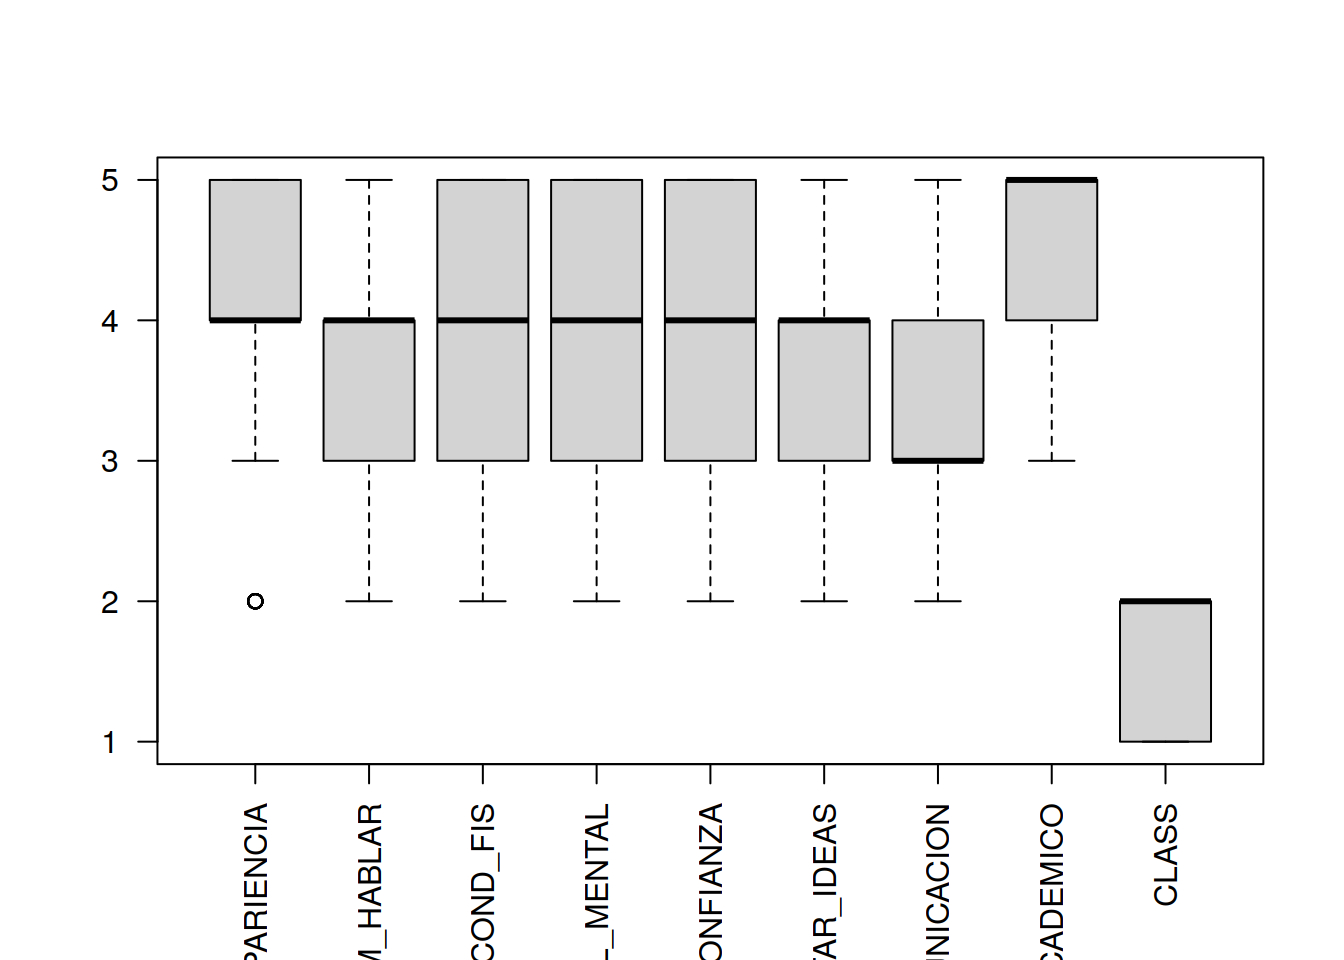
\includegraphics[width=0.8\textwidth]{grafico_cajas}
    \caption{Gráficos de cajas de las variables de entrada}
\end{figure}

A la hora de borrar \textit{outliers}, de forma univariante, solo la variable \textit{Apariencia} los presenta. Concretamente, presenta 14 registros, lo que supone un 0.587\% del total de los registros, por que lo borramos dichos registros. Aplicando la misma transformación de datos, para no caer en \textit{data snooping}, borramos 2 filas en test, lo que supone un 0.335\%.

A la hora de borrar \textit{outliers}, de forma multivariante, borramos 13 filas del conjunto de entrenamiento, lo que supone un 0.084\%. Para no caer en \textit{data snooping}, no aplicamos este borrado usando la distancia \textit{Mahalanobis} sobre el conjunto de \textit{test}.

En \customref{fig:balanceo_clases} ya hemos visto el balanceo de las clases, con aproximadamente un 60\% de no empleables, 40\% de empleables.

El estudio de la normalidad univariante, apoyado en los gráficos \textit{qqplot} y el contraste de hipótesis nos muestra que \textbf{no tenemos normalidad univariante}, de forma muy contundente. Los gráficos \textit{qqplot} obtenidos son los siguientes:

\begin{figure}[H]
    \centering
    \begin{subfigure}{0.45\textwidth}
    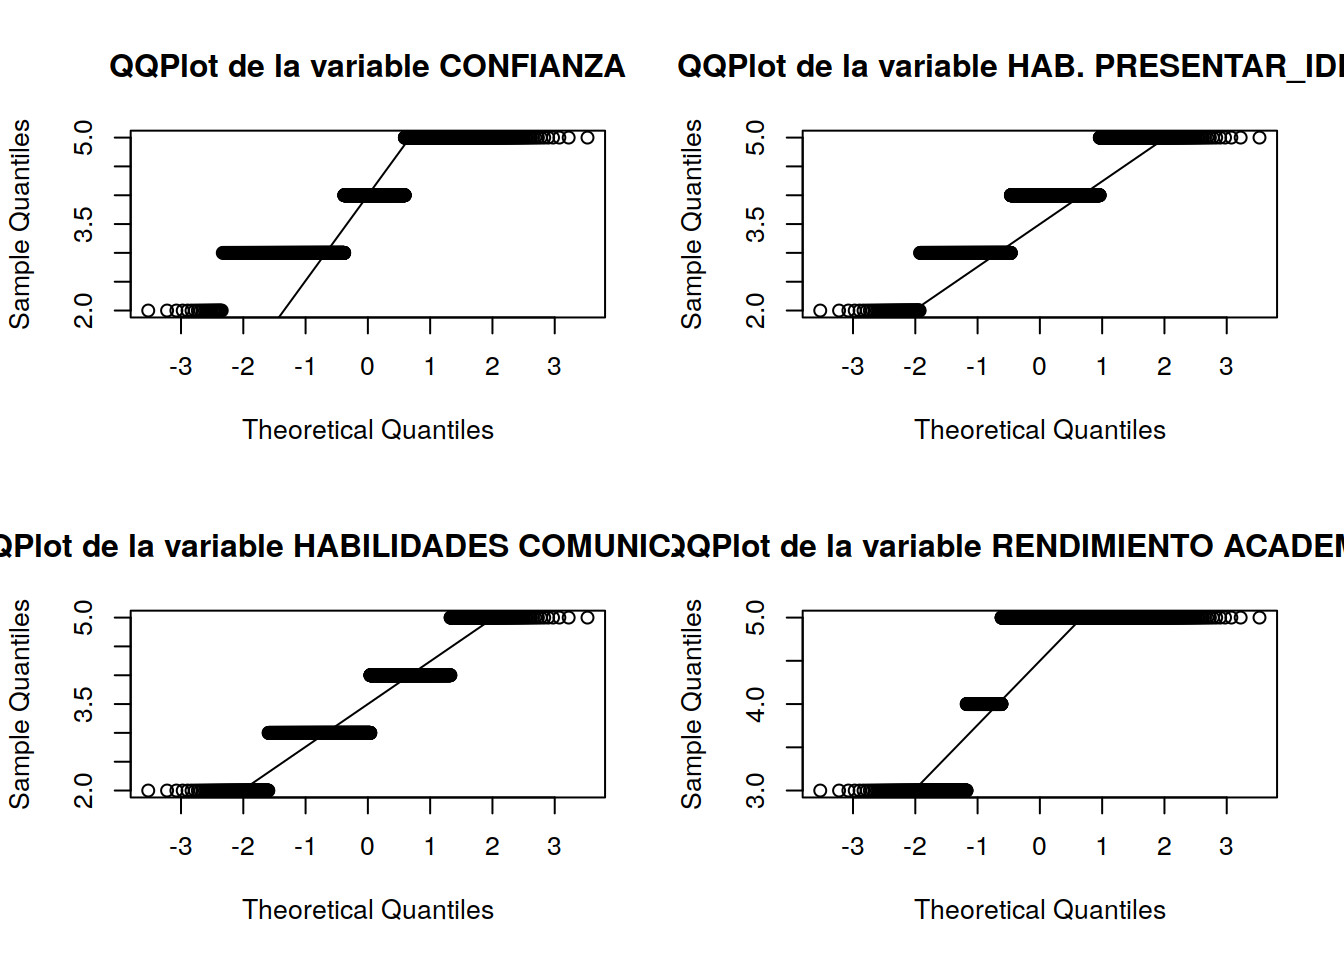
\includegraphics[width=1.0\textwidth]{graficos_qqplot}
    \end{subfigure}
    \begin{subfigure}{0.45\textwidth}
        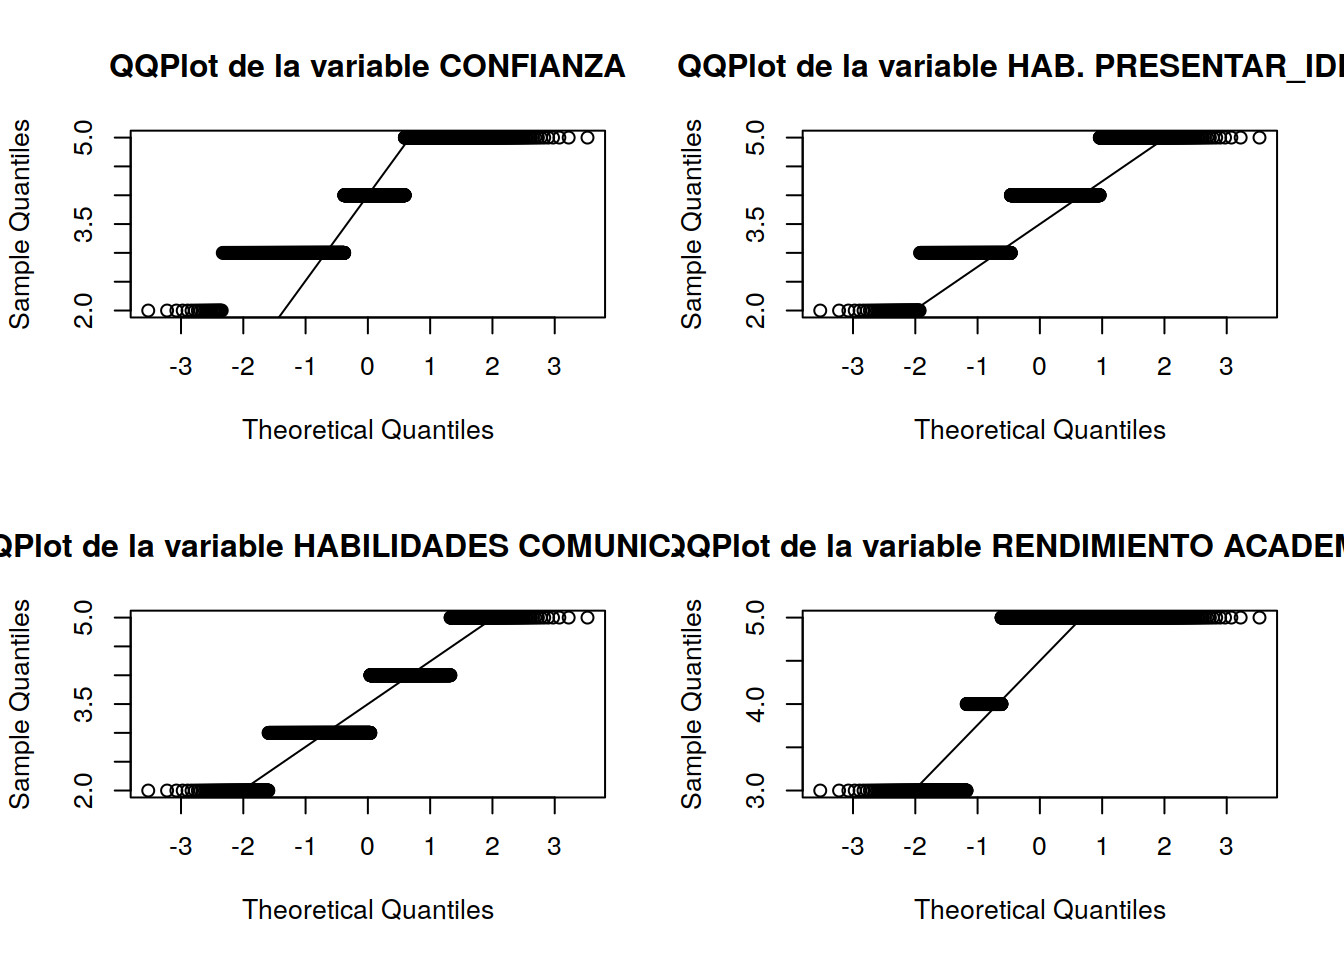
\includegraphics[width=1.0\textwidth]{graficos_qqplot_segunda}
    \end{subfigure}

    \caption{Gráficos \textit{qqplot} de las variables de entrada}
\end{figure}

La visualización de la matriz de correlaciones, junto con el \textit{test de esfericidad de Bartlett} nos dejan claro que las variables están correlacionadas. La matriz de correlaciones se muestra como la siguiente visualización:

\begin{figure}[H]
    \centering
    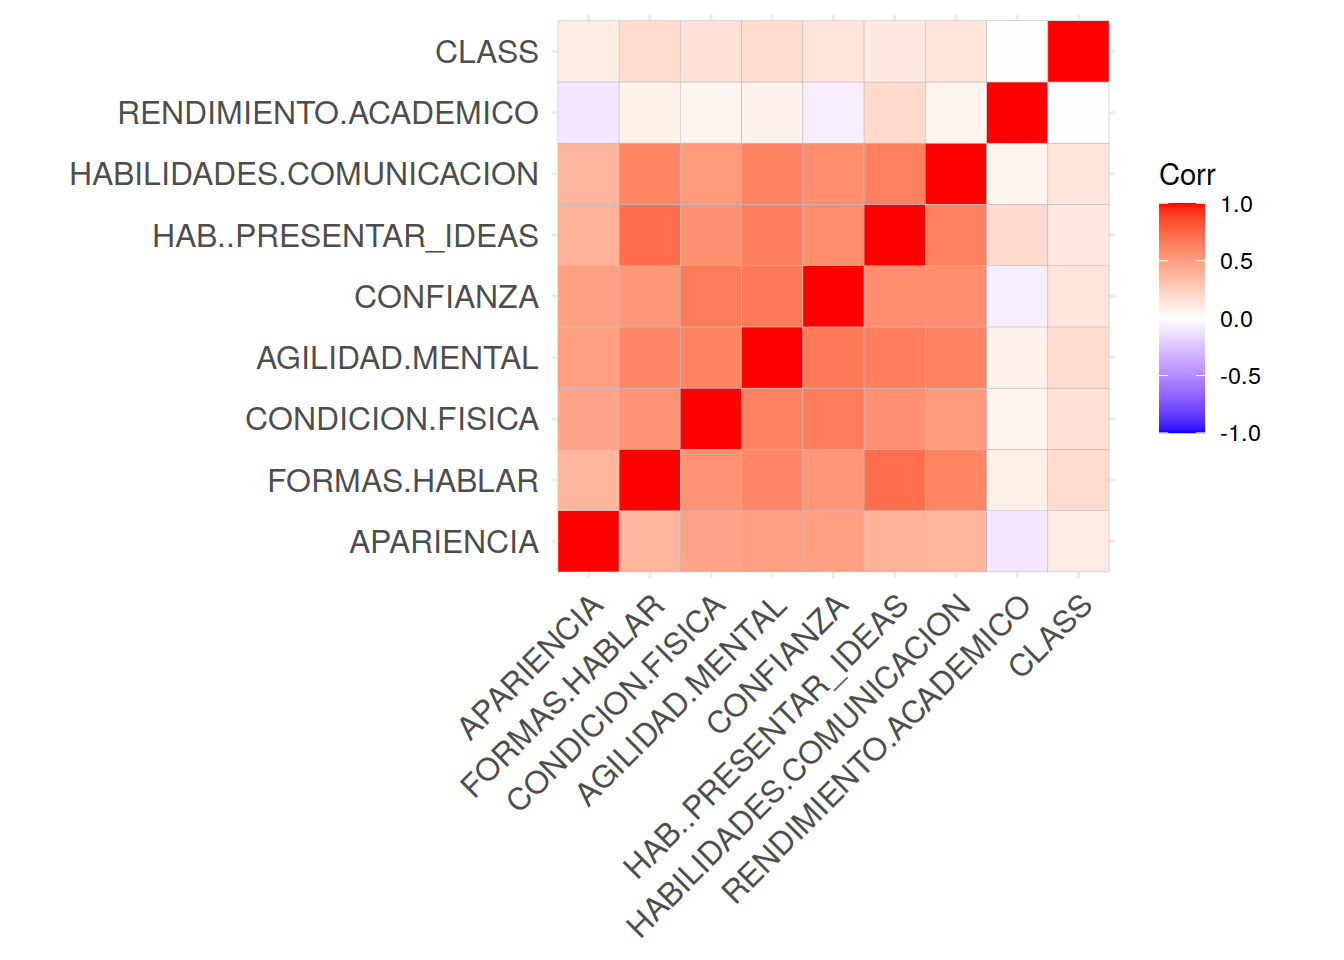
\includegraphics[width=0.8\textwidth]{matriz_correlaciones}
    \caption{Matriz de correlaciones}
\end{figure}

Podemos visualizar, en otro formato, los pares de variables que más correladas están entre sí:

\begin{figure}[H]
    \centering
    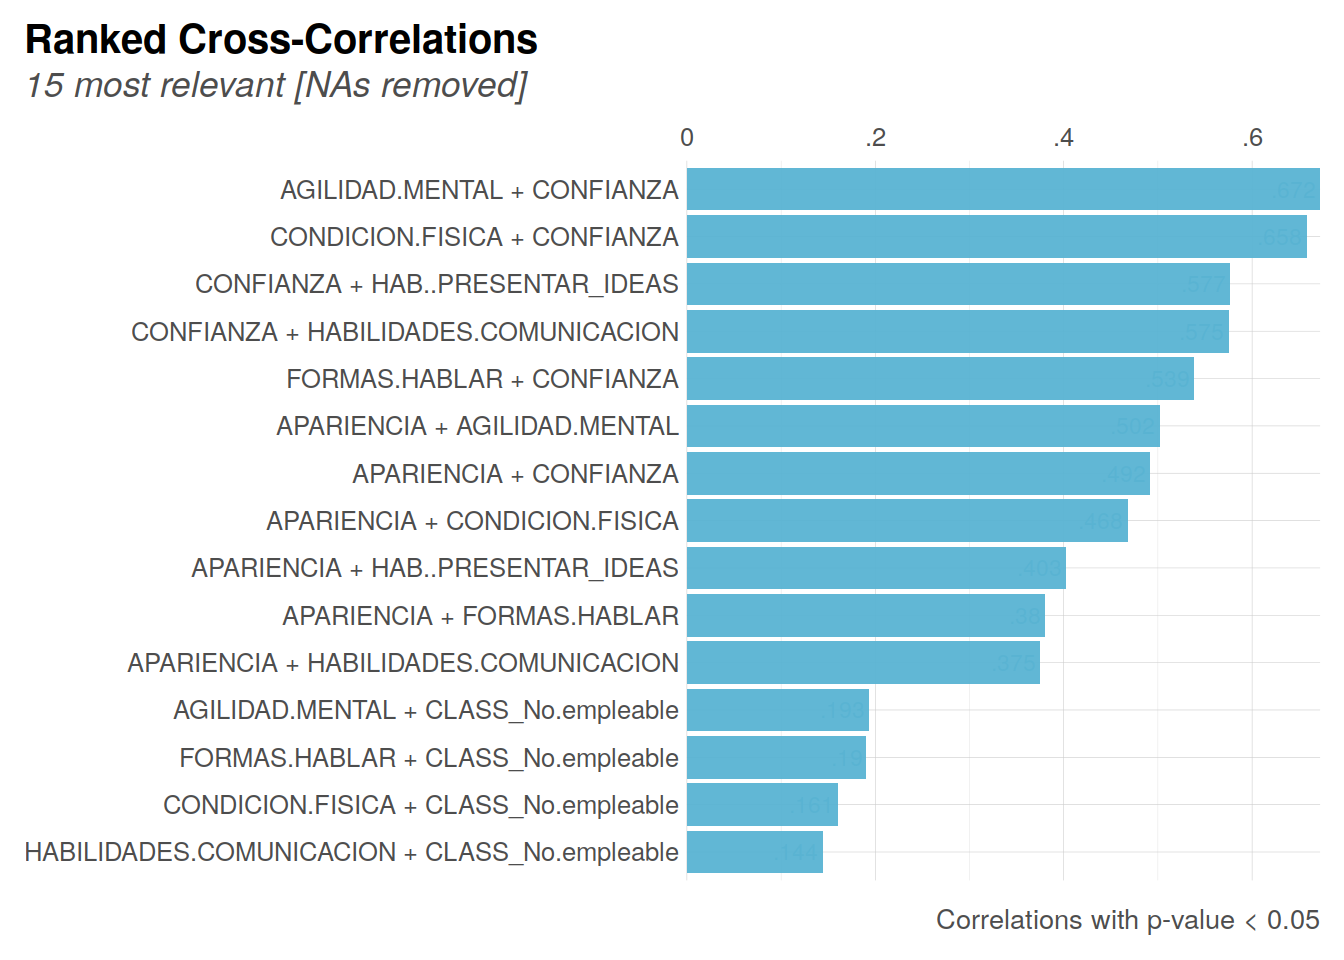
\includegraphics[width=0.8\textwidth]{rank_correlaciones}
    \caption{Pares de variables más correladas entre sí}
\end{figure}

Y también, podemos ver esto mismo en dos subconjuntos de datos, el de registros asociados a personas empleables y el de no empleables:

\begin{figure}[H]
    \centering
    \begin{subfigure}{0.45\textwidth}
        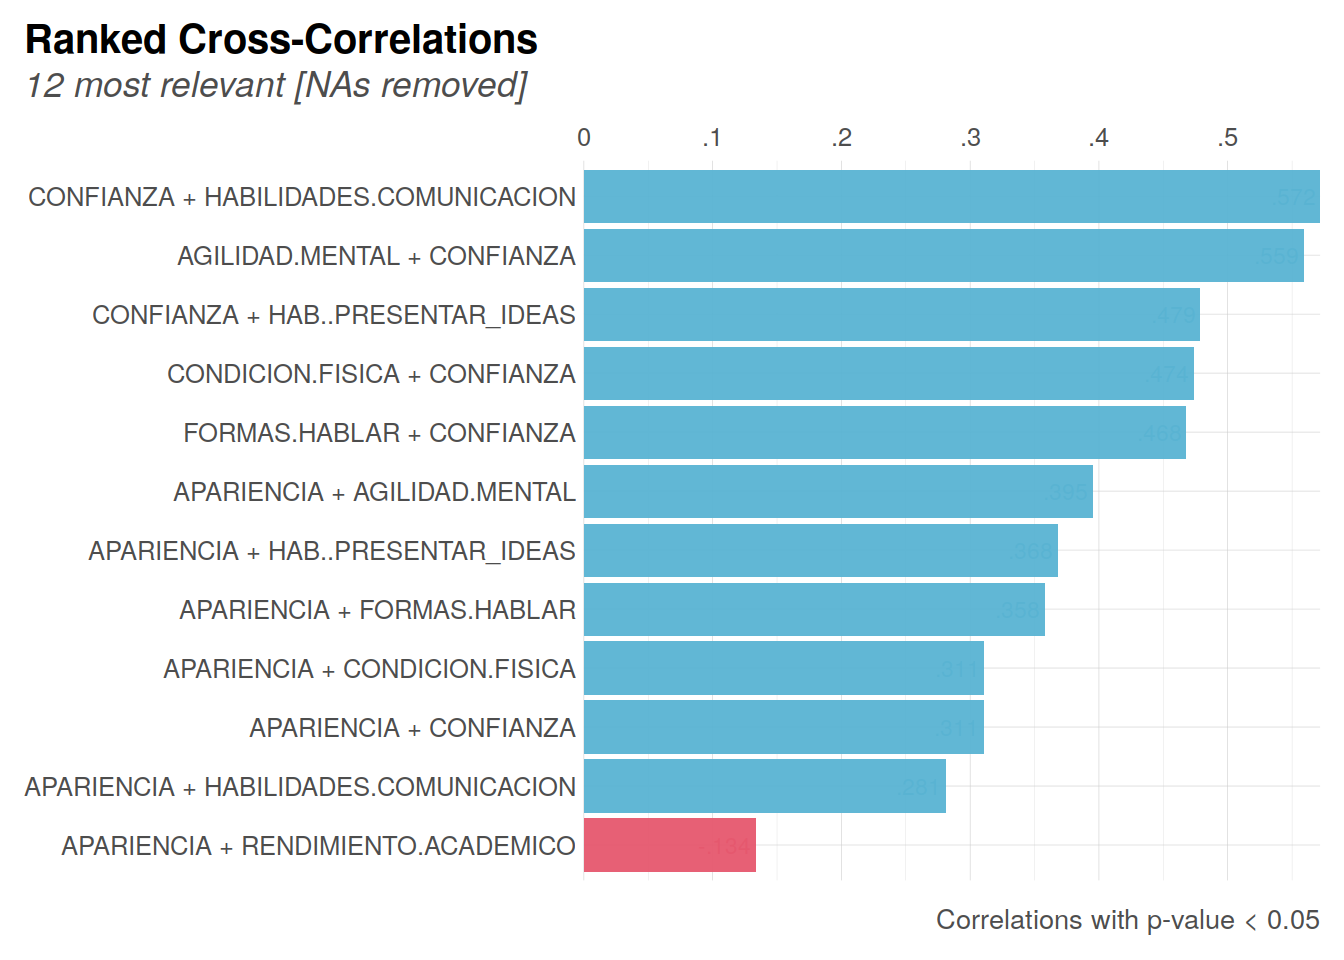
\includegraphics[width=1.0\textwidth]{rank_empleables}
        \caption{Candidatos empleables}
    \end{subfigure}
    \begin{subfigure}{0.45\textwidth}
        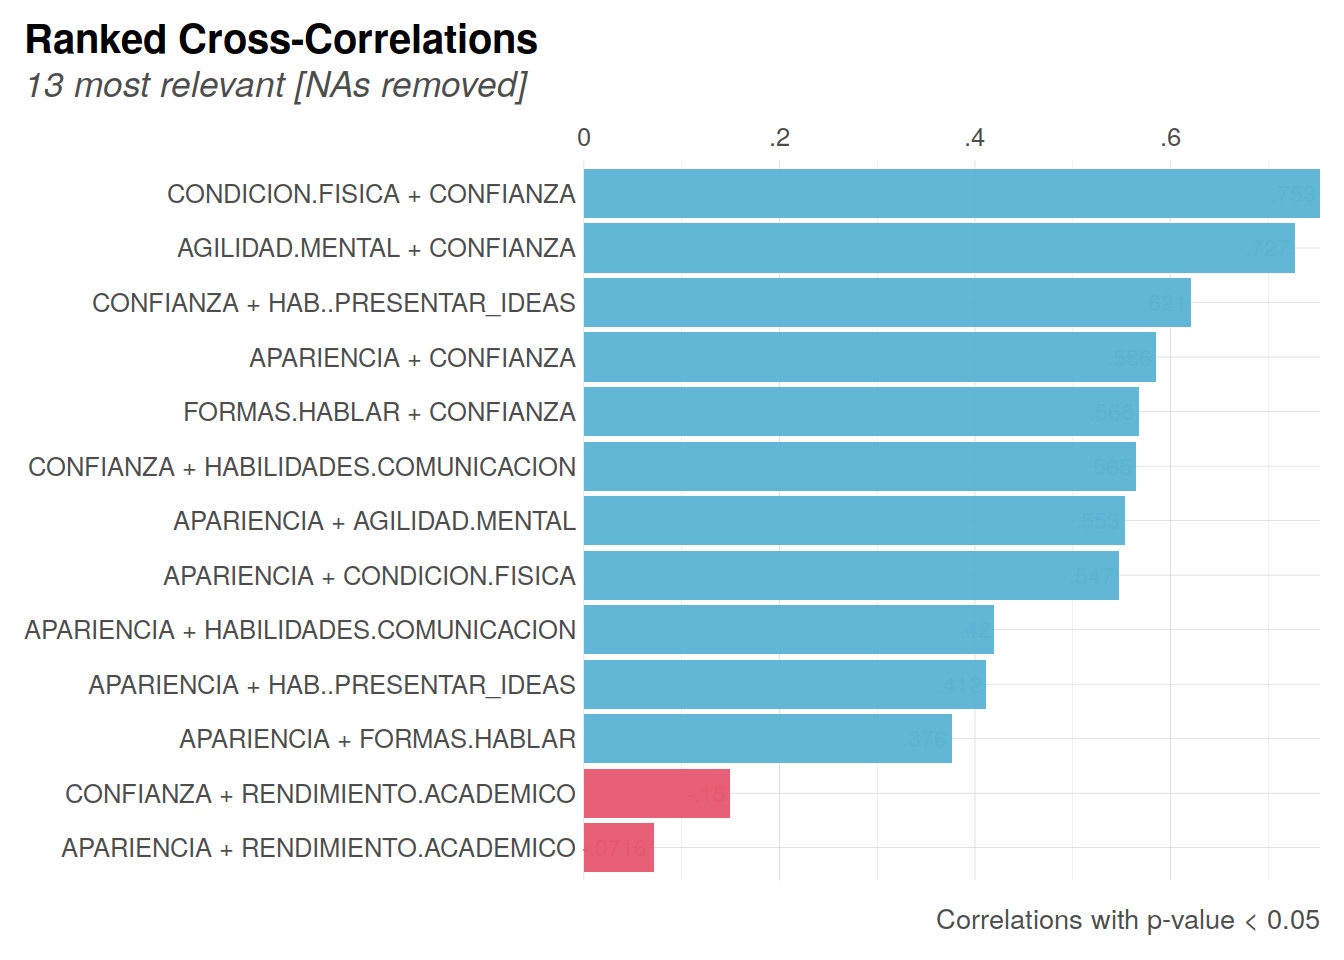
\includegraphics[width=1.0\textwidth]{rank_no_empleables}
        \caption{Candidatos no empleables}
    \end{subfigure}

    \caption{Pares de variables más correladas entre sí, según la empleabilidad}
\end{figure}

Los contrastes de hipótesis, que ya hemos comentado, nos indican que \textbf{NO tenemos normalidad multivariante}, como era de esperar al fallar la normalidad univariante.

Otro contraste de hipótesis nos indica que \textbf{NO tenemos homogeneidad de la varianza}. Aunque al fallar la normalidad multivariante, este resultado no es fiable. No es del todo relevante que el \textit{test} no sea fiable. Puesto que estamos comprobando los supuestos para los modelos discriminante, y la falta de normalidad ya hace que, independientemente de la homogeneidad de la varianza, no vayan a funcionar de forma óptima.

Por tanto, los dos \textbf{supuestos sobre los que se sustentan el discriminante lineal y cuadrático fallan}.


\subsection{Reducción de la dimensionalidad}

Esta parte es muy relevante en nuestro estudio. Porque producimos dos nuevos conjuntos de datos, que proporcionarán uno de los mejores resultados a la hora de clasificar, y porque además serán muy relevantes a la hora de estudiar la posible falta de meritocracia.

Además, mantenemos a partir de ahora tres conjuntos de datos:

\begin{enumerate}
    \item El conjunto de datos original, sobre el que realizamos el tratamiento ya mencionado
    \item El conjunto de datos original al que aplicamos \textit{PCA}
    \item El conjunto de datos original al que aplicamos \textit{FA}
\end{enumerate}

Esto porque a la hora de clasificar, tenemos que elegir todavía cuál es la mejor combinación de modelo-conjunto de datos. Y no todos los modelos necesariamente tengan los mejores resultados sobre el mismo conjunto de datos.

\subsubsection{Componentes Principales}

Veamos la varianza explicada, y la varianza explicada acumulada, por las componentes principales:

\begin{figure}[H]
    \centering
    \begin{subfigure}{0.45\textwidth}
        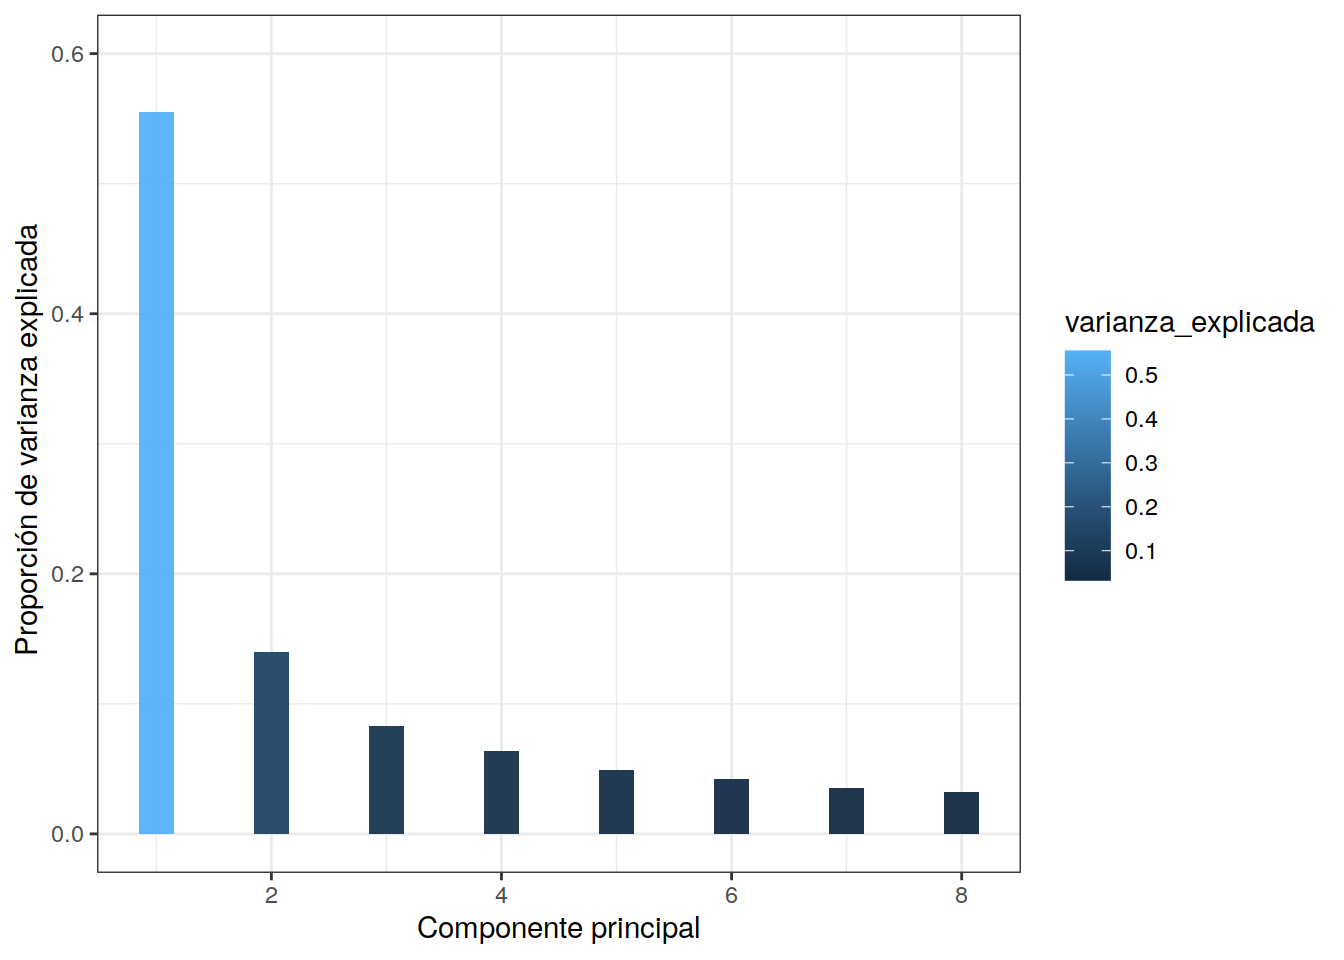
\includegraphics[width=1.0\textwidth]{pca_var_explicada}
        \caption{Proporción de la varianza explicada por las componentes principales}
    \end{subfigure}
    \begin{subfigure}{0.45\textwidth}
        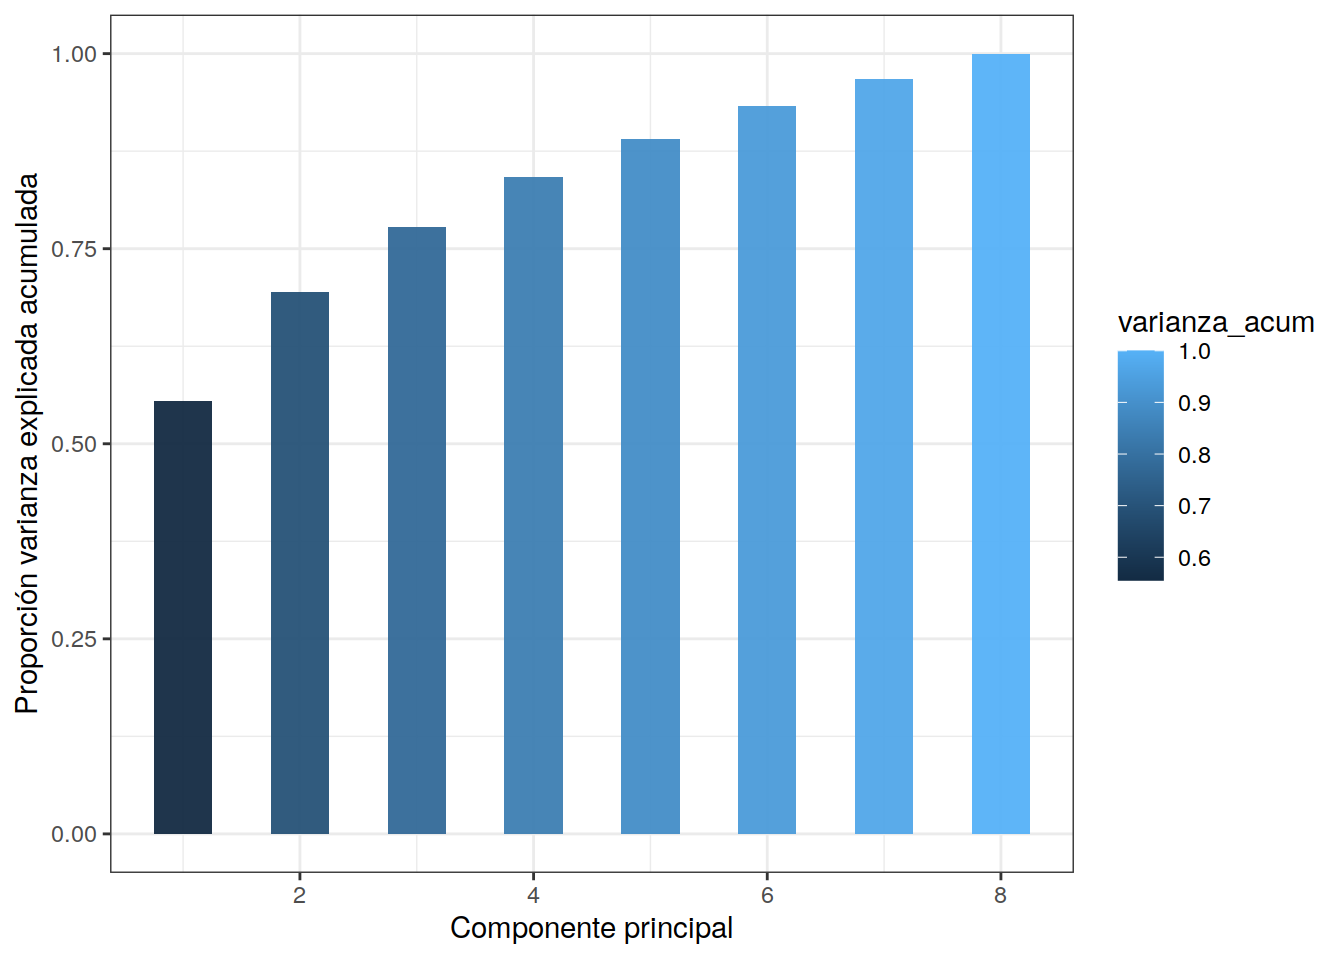
\includegraphics[width=1.0\textwidth]{pca_var_explicada_acumulada}
        \caption{Proporción de la varianza explicada acumulada por las componentes principales}
    \end{subfigure}

    \caption{Información sobre la proporción de la varianza explicada por cada una de las componentes principales}
\end{figure}

Los resultados de los métodos para elegir el número de componentes principales son:

\begin{itemize}
    \item Regla de \textit{Abdi}: dos componentes
    \item Mínimo de Varianza explicada: cuatro componentes, buscando explicar al menos el 80\% de la varianza
    \item Método del codo: dos componentes
    \item Análisis paralelo: dos componentes
\end{itemize}

El método del codo y análisis paralelo se fundamentan en los siguientes gráficos:

\begin{figure}[H]
    \centering
    \begin{subfigure}{0.45\textwidth}
        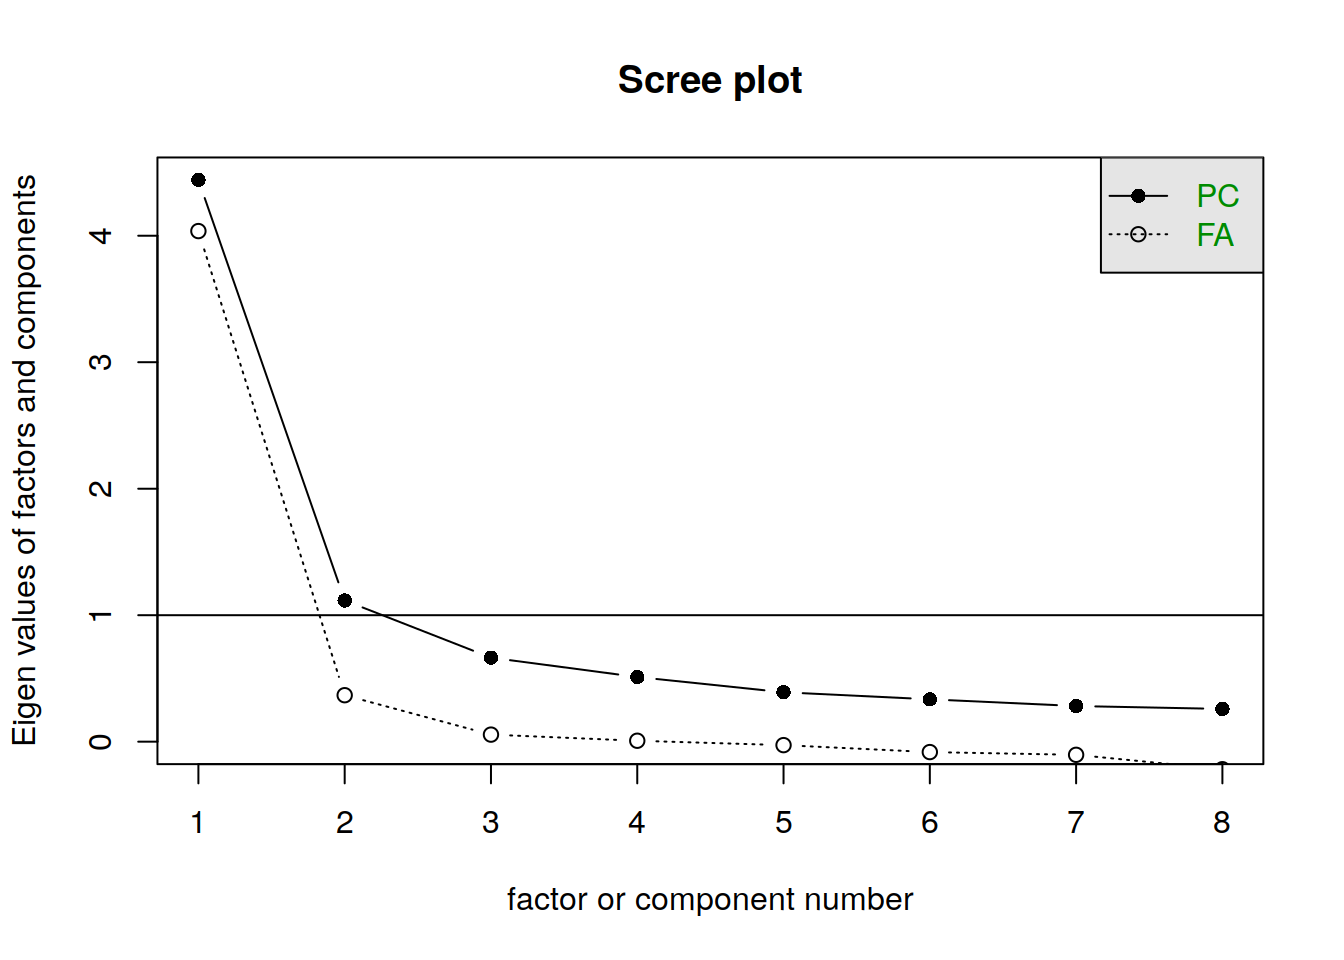
\includegraphics[width=1.0\textwidth]{pca_codo}
        \caption{Gráfica del método del codo}
    \end{subfigure}
    \begin{subfigure}{0.45\textwidth}
        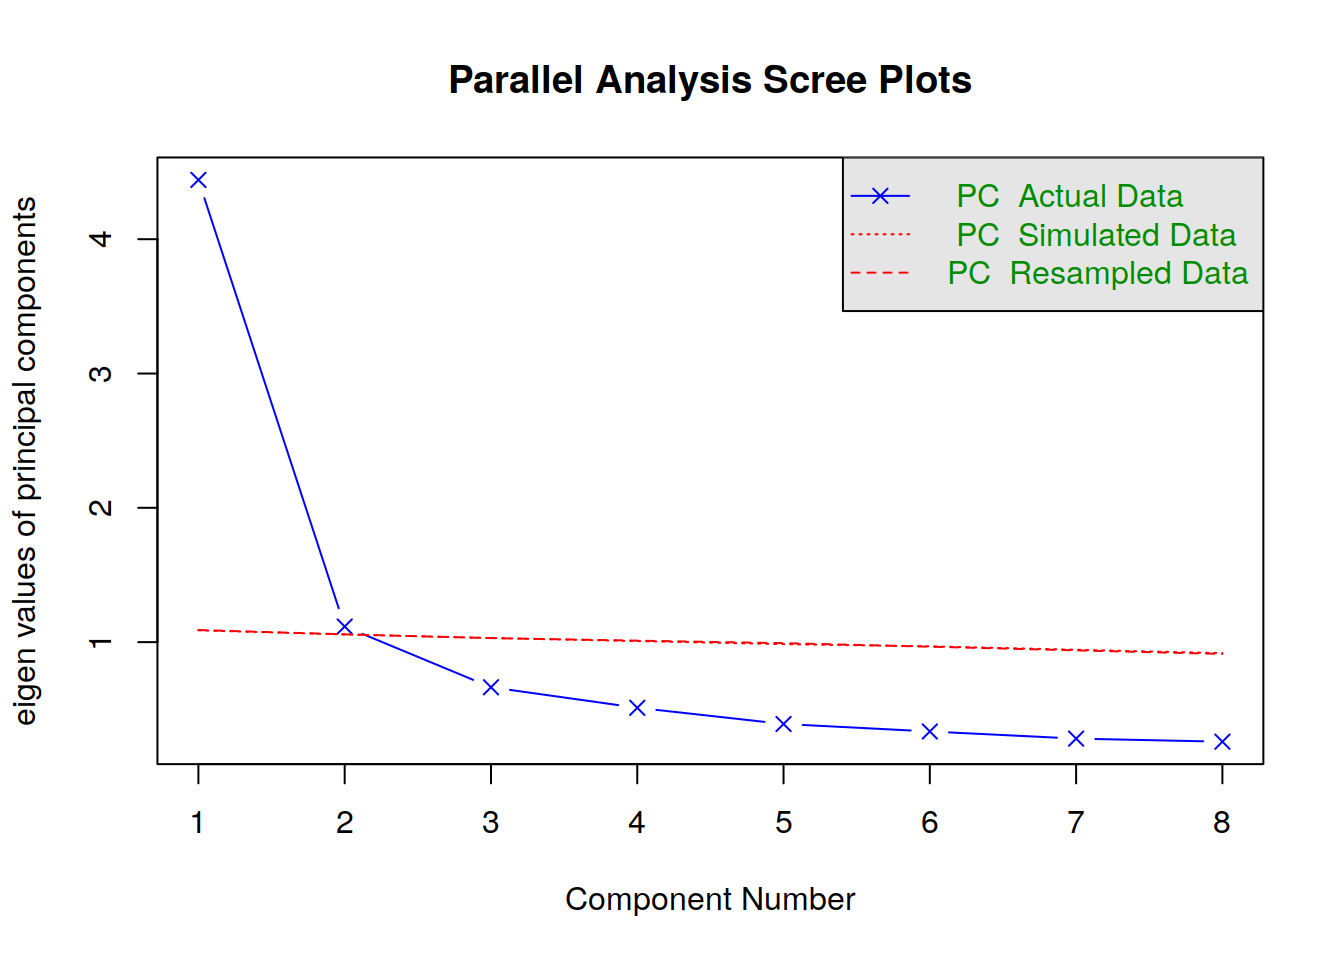
\includegraphics[width=1.0\textwidth]{pca_paralelo}
        \caption{Gráfica para el método paralelo}
    \end{subfigure}

    \caption{Gráficas sobre las que se fundamentan el método del codo y método del análisis paralelo}
\end{figure}

Por tanto, elegimos usar \textbf{dos componentes principales}

Tras realizar la transformación de los datos, podemos mostrar el siguiente gráfico:

\begin{figure}[H]
    \centering
    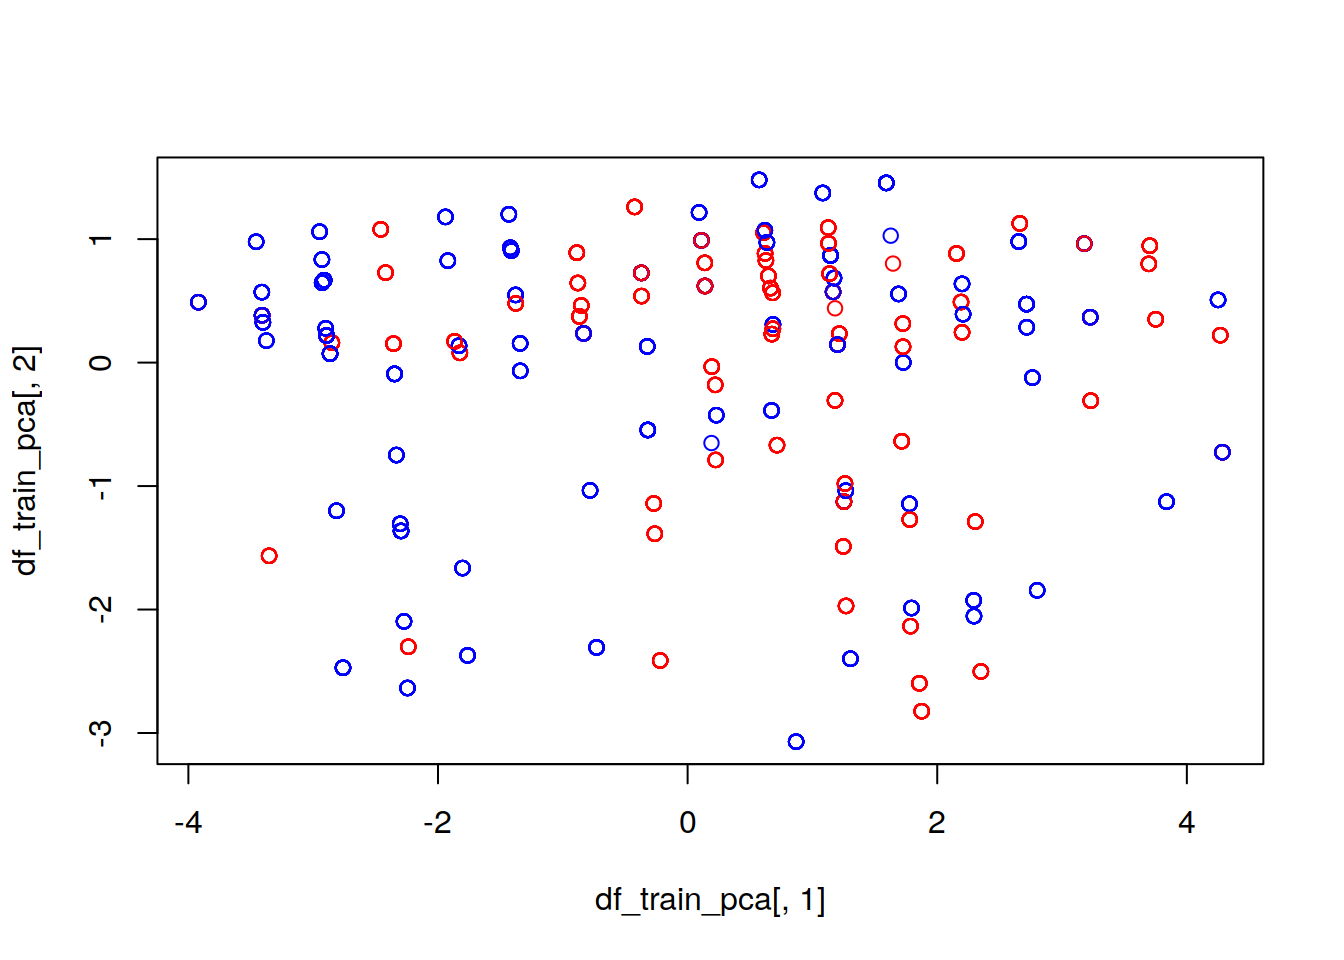
\includegraphics[width=0.60\textwidth]{scatter_plot_pca}
    \caption{Dos primeras componentes principales, coloreadas según la empleabilidad}
\end{figure}

Además, podemos visualizar la relevancia de las variables de entrada a la hora de generar las dos componentes principales:

\begin{figure}[H]
    \centering
    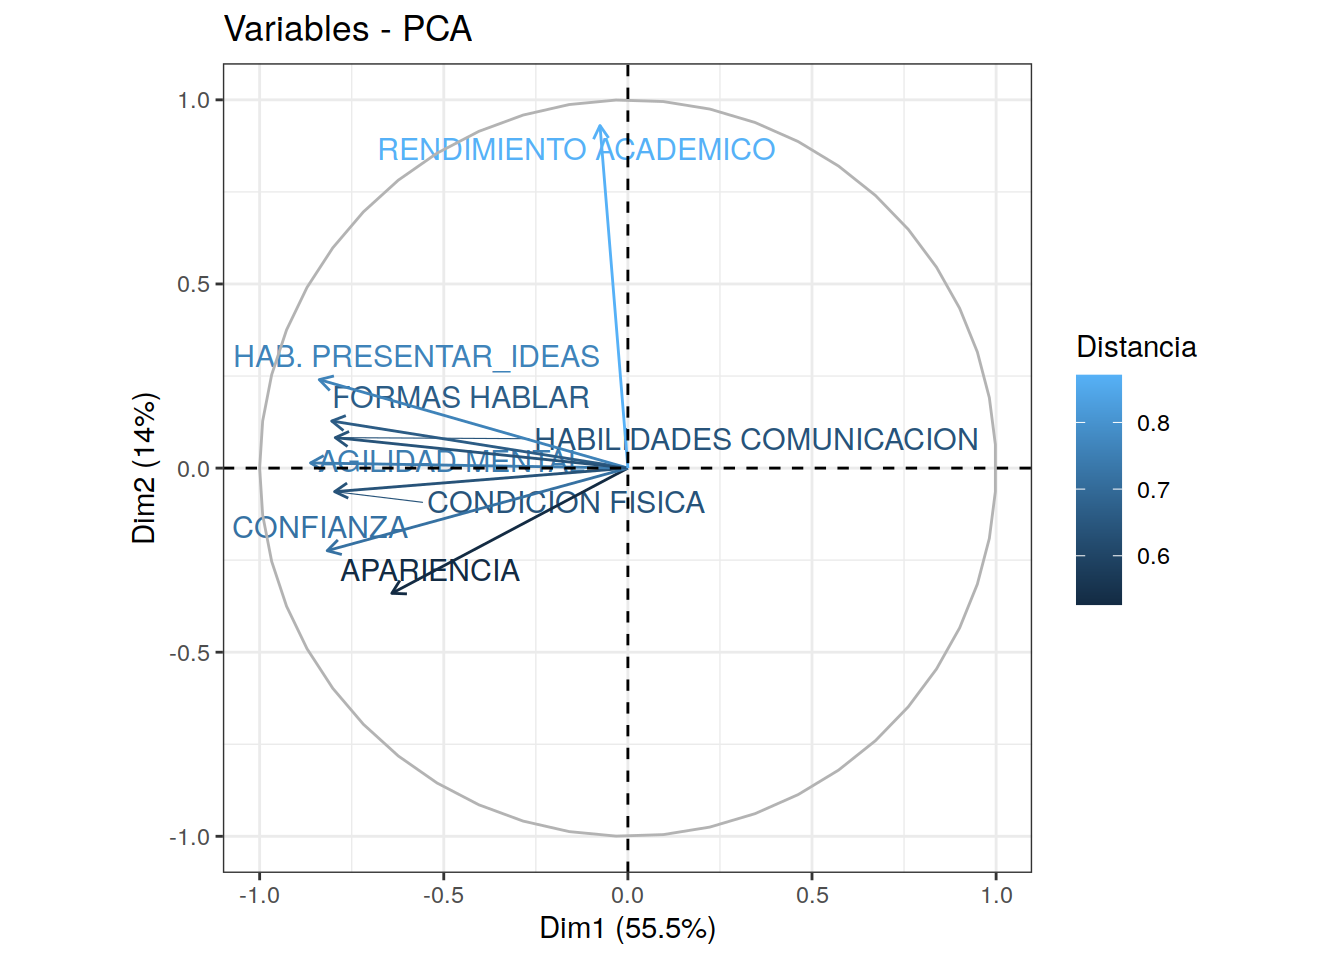
\includegraphics[width=0.8\textwidth]{pca_ejes}
    \caption{Importancia de las variables de entrada a la hora de calcular las dos primeras componentes principales}
\end{figure}

\subsubsection{Análisis Factorial}


Los resultados de los métodos para elegir el número de variables latentes son:

\begin{itemize}
    \item Método del codo: un factor latente
    \item Análisis paralelo: dos factores latentes
\end{itemize}

Esto se fundamenta en los siguientes gráficos:

\begin{figure}[H]
    \centering
    \begin{subfigure}{0.45\textwidth}
        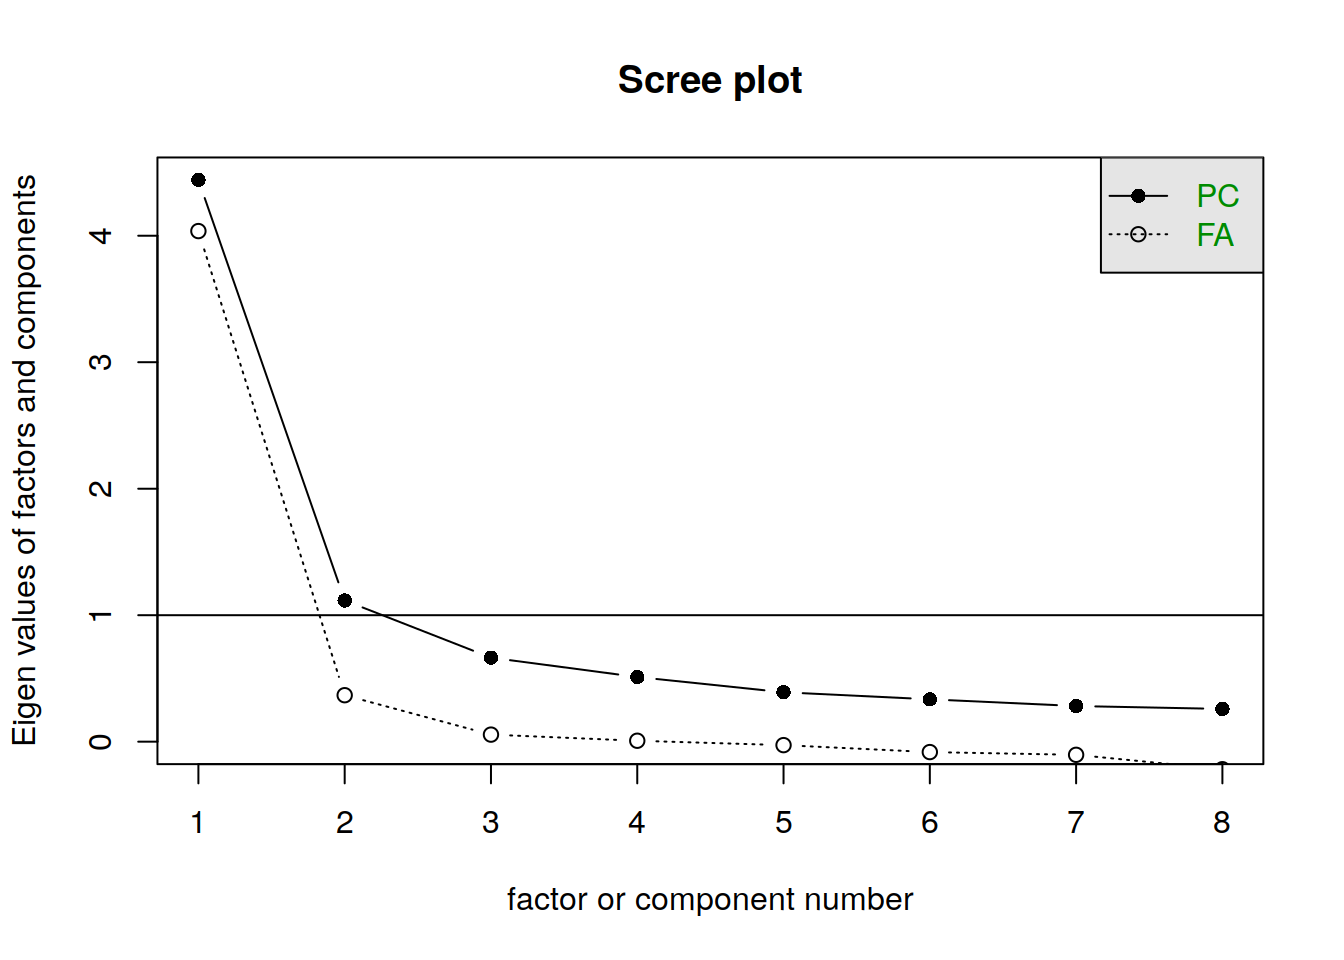
\includegraphics[width=1.0\textwidth]{fa_codo}
        \caption{Gráfica del método del codo}
    \end{subfigure}
    \begin{subfigure}{0.45\textwidth}
        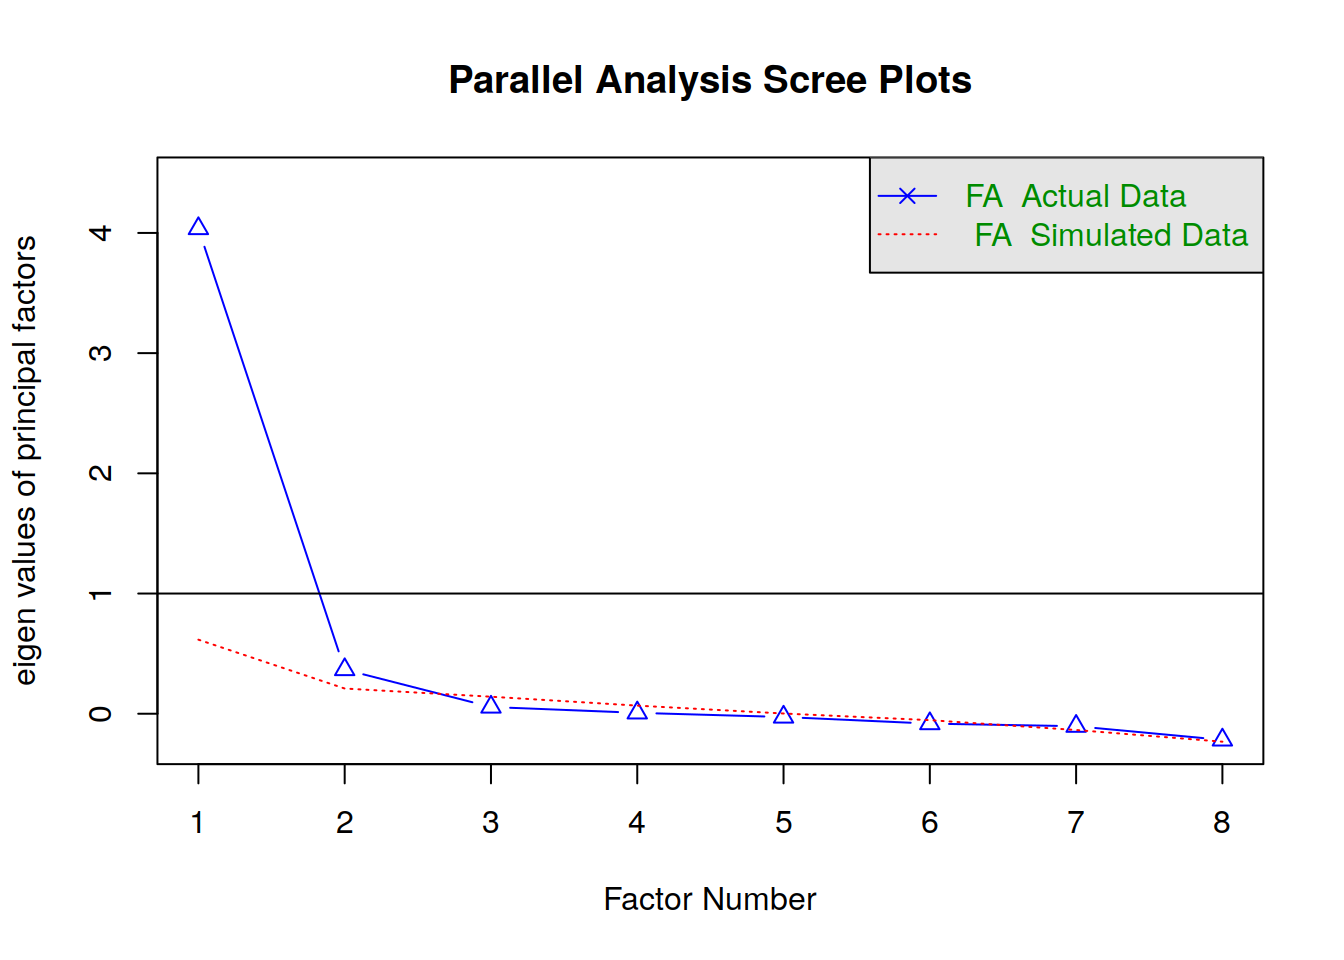
\includegraphics[width=1.0\textwidth]{fa_paralelo}
        \caption{Gráfica para el método paralelo}
    \end{subfigure}

    \caption{Gráficas sobre las que se fundamentan el método del codo y método del análisis paralelo}
\end{figure}

Con un contraste de hipótesis, vemos que es suficiente con un factor latente, y por tanto, también con dos factores latentes. Podemos visualizar cómo se construyen las variables latentes, tanto en el caso de una o dos variables latentes:

\begin{figure}[H]
    \centering
    \begin{subfigure}{0.45\textwidth}
        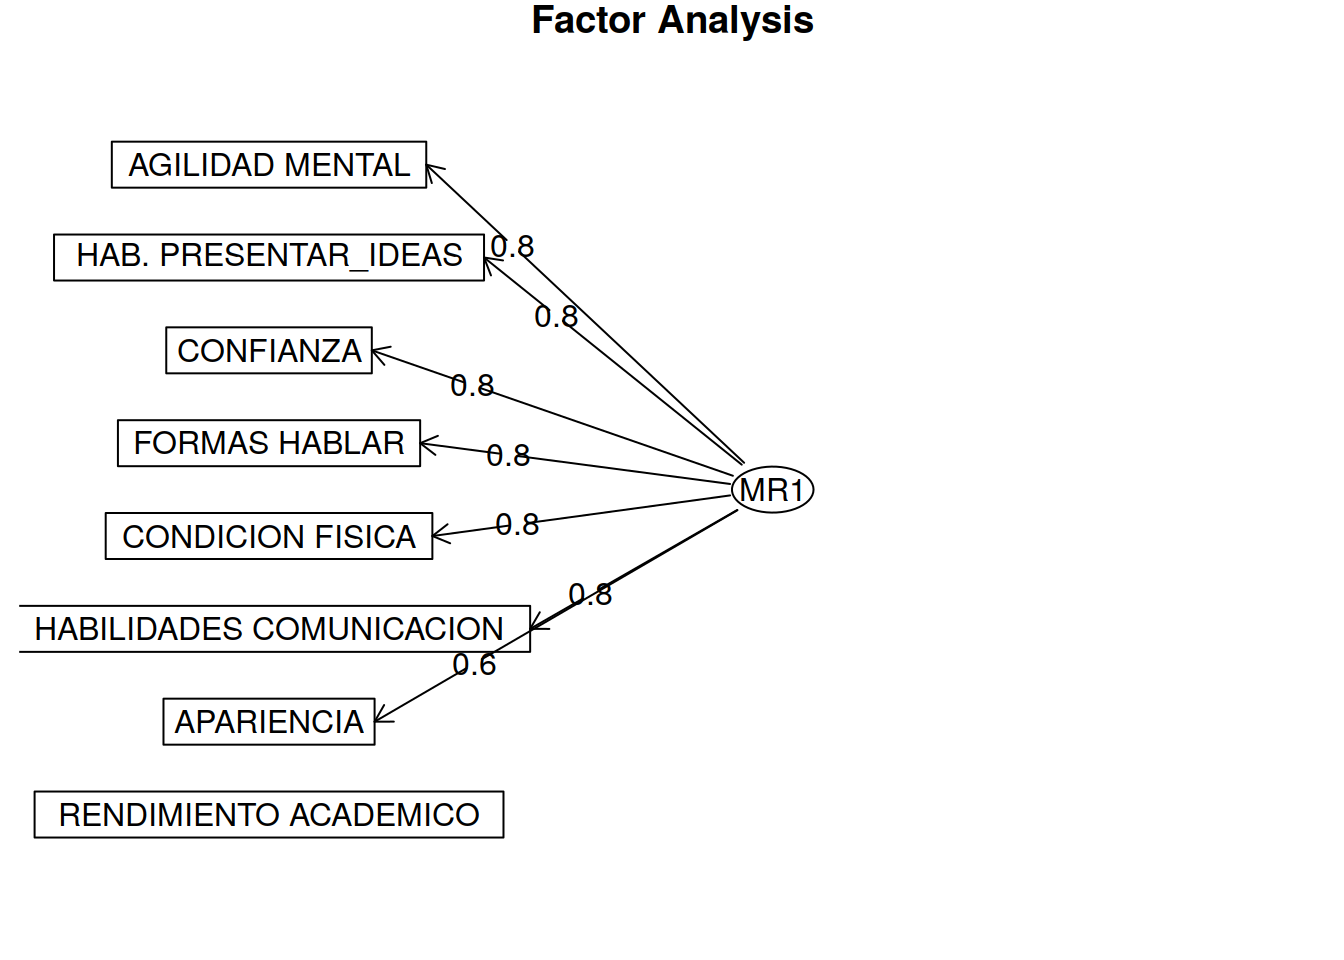
\includegraphics[width=1.0\textwidth]{var_latentes_uno}
        \caption{Combinación de las variables de entrada, para un solo factor latente}
    \end{subfigure}
    \begin{subfigure}{0.45\textwidth}
        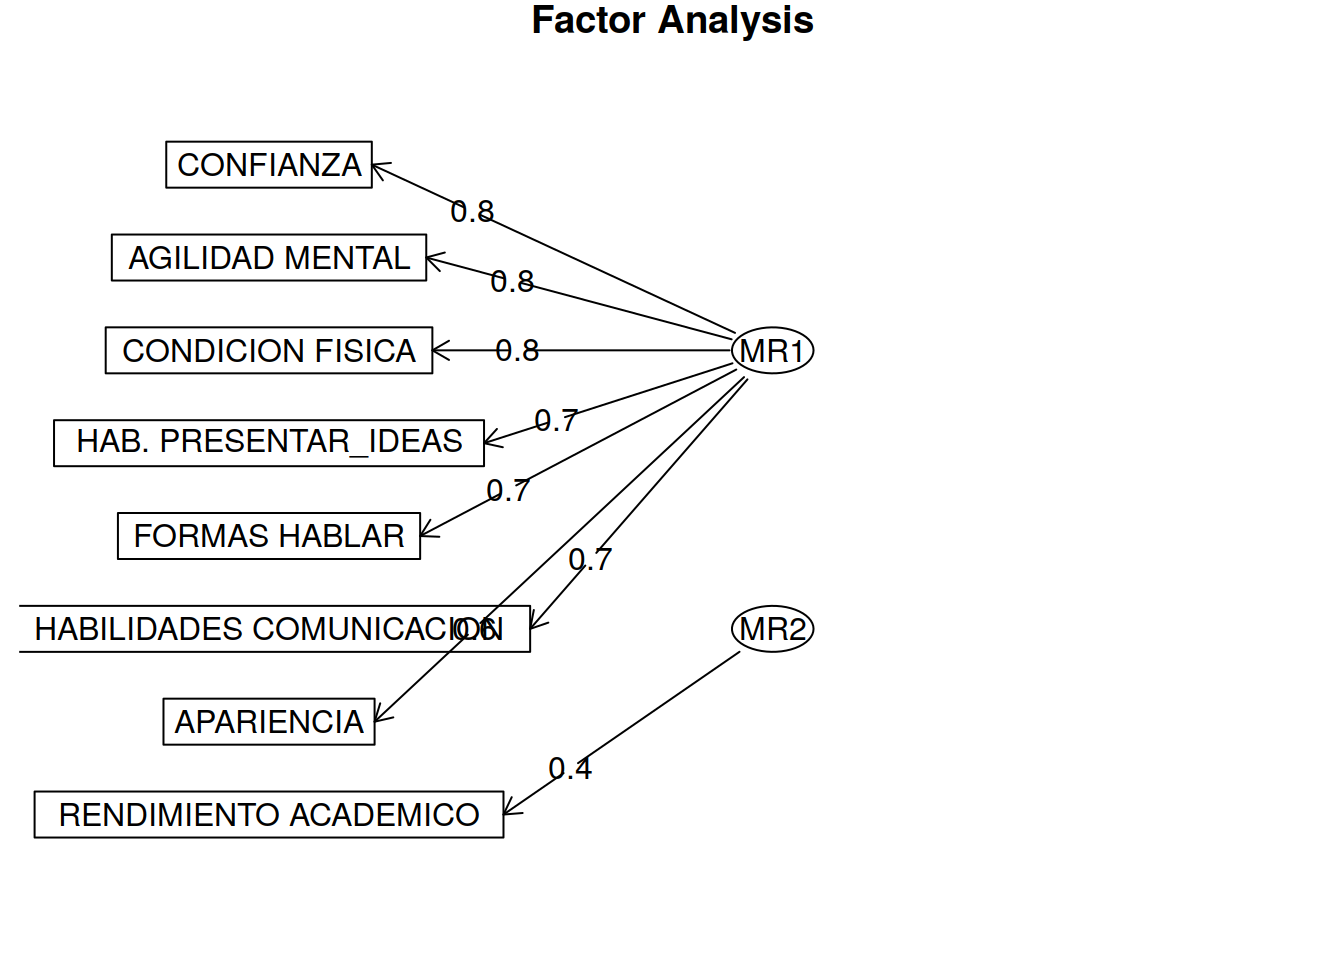
\includegraphics[width=1.0\textwidth]{var_latentes_dos}
        \caption{Combinación de las variables de entrada, para dos factores latentes}
    \end{subfigure}

    \caption{Gráfica que muestra cómo se combinan las variables para calcular los factores latentes, para un solo factor latente y para dos factores latentes}
\end{figure}

Por los motivos que comentamos en \customref{section:Discusion}, al final decidimos quedarnos con dos variables latentes, aunque sea suficiente con una variable latente.

\subsection{Exploración de hiperparámetros}

\textit{XGBOOST} tiene hiperparámetros que podemos optimizar usando \textit{k-Fold Cross Validation}. Sin embargo, por la potencia del modelo, basta con que usemos unos parámetros que consideramos razonables, y los modificamos ligeramente para obtener el resultado final. Usamos los siguientes hiperparámetros en este modelo:

\begin{itemize}
    \item \lstinline{max_depth} = 10
    \item \lstinline{eta} = 0.3
    \item \lstinline{nrounds} = 100
\end{itemize}

Los resultados se resumen en la siguiente tabla:

\begin{table}[H]
\centering
\begin{tabular}{|l|l|l|}
    \hline
    Modelo                   & Dataset      & Accuracy      \\
    \hline
    Discriminante Lineal     & Original     & 0.5915605     \\
    Discriminante Lineal     & PCA          & 0.5334985     \\
    Discriminante Lineal     & FA           & 0.5284333     \\
    Discriminante Cuadrático & Original     & 0.6891568     \\
    Discriminante Cuadrático & PCA          & 0.5615132     \\
    Discriminante Cuadrático & FA           & 0.587775      \\
    XGBOOST                  & Original     & 0.9014924     \\
    \textbf{XGBOOST}         & \textbf{PCA} & \textbf{0.9046639} \\
    XGBOOST                  & FA           & 0.9036134     \\
    \hline

\end{tabular}
\caption{Resultados de \textit{k-Fold Cross Validation}}
\label{table:cross_validation}
\end{table}

Vemos que los mejores resultados se obtienen con \textit{XGBOOST} sobre el conjunto de \textit{PCA}. El discriminante cuadrático y el discriminante lineal obtienen sus mejores resultados sobre el conjunto de datos original.

\subsection{Clasificación}

Aunque \textbf{ya hemos decidido que el mejor modelo es \textit{XGBOOST}} sobre los datos a los que aplicamos \textit{PCA}, entrenamos y validamos los tres modelos, cada uno con el conjunto de datos sobre el que obtiene mejores resultados. Con esto, \textbf{podemos realizar un estudio sobre el comportamiento de los tres modelos}.

Los coeficientes (en valor absoluto) del discriminante lineal, que discutiremos en \customref{section:Discusion}, se visualizan en la siguiente figura:

\begin{figure}[H]
    \centering
    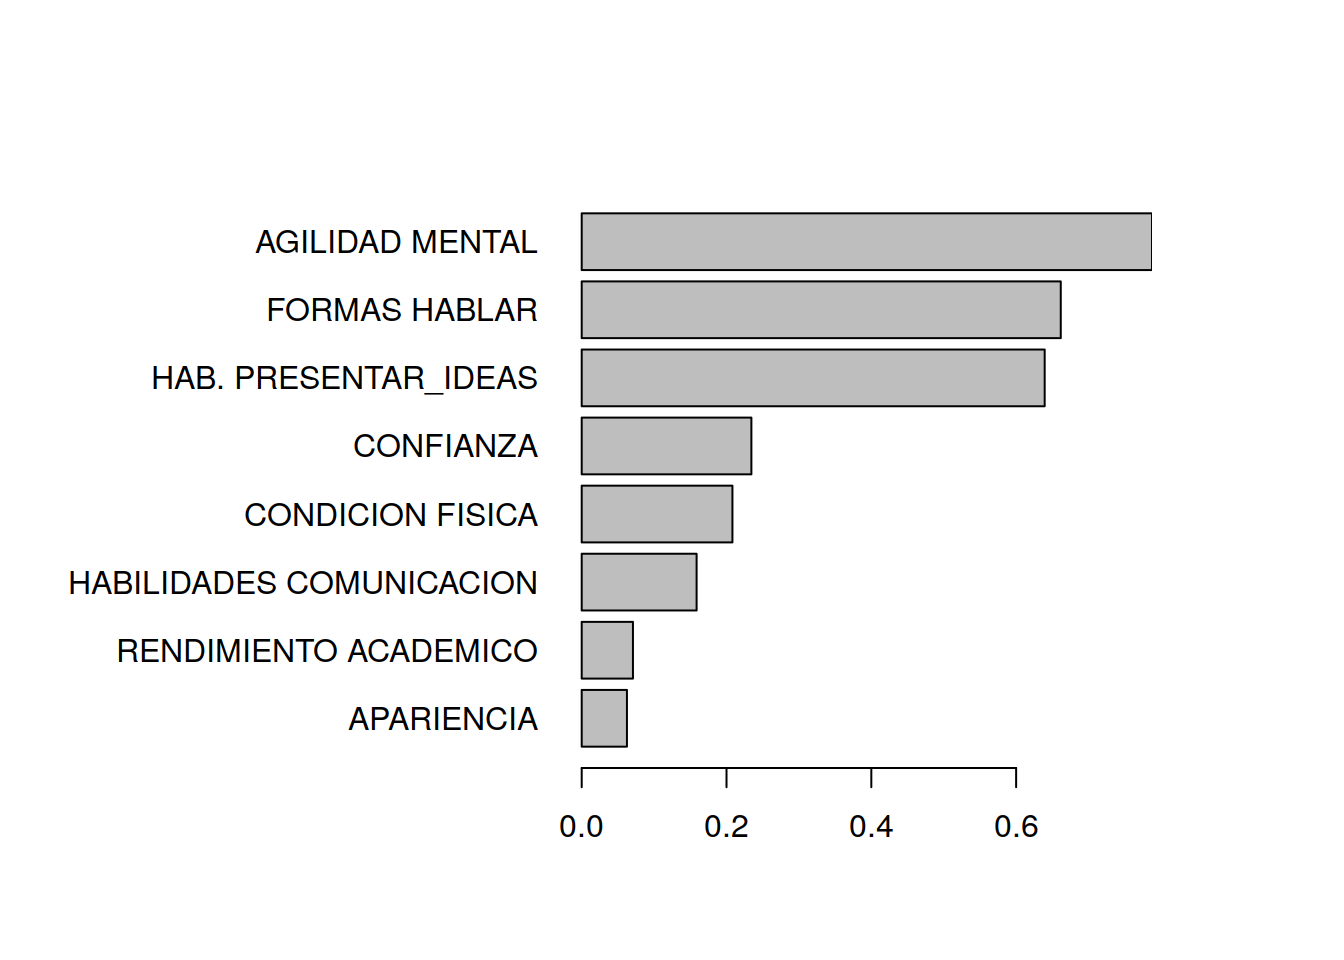
\includegraphics[width=0.8\textwidth]{coeficientes_lda}
    \caption{Visualización de los valores absolutos de los coeficientes del modelo discriminante lineal}
\end{figure}

El paquete de \textit{XGBOOST} nos otorga una función para mostrar la importancia de cada variable. Mostramos dicha importancia, tanto para el modelo sobre \textit{PCA} (que es el que escogemos por lo visto en \customref{table:cross_validation}) como para el modelo sobre el conjunto de datos original (que solo usamos para visualizar dicha relevancia):

\begin{figure}[H]
    \centering
    \begin{subfigure}{0.45\textwidth}
        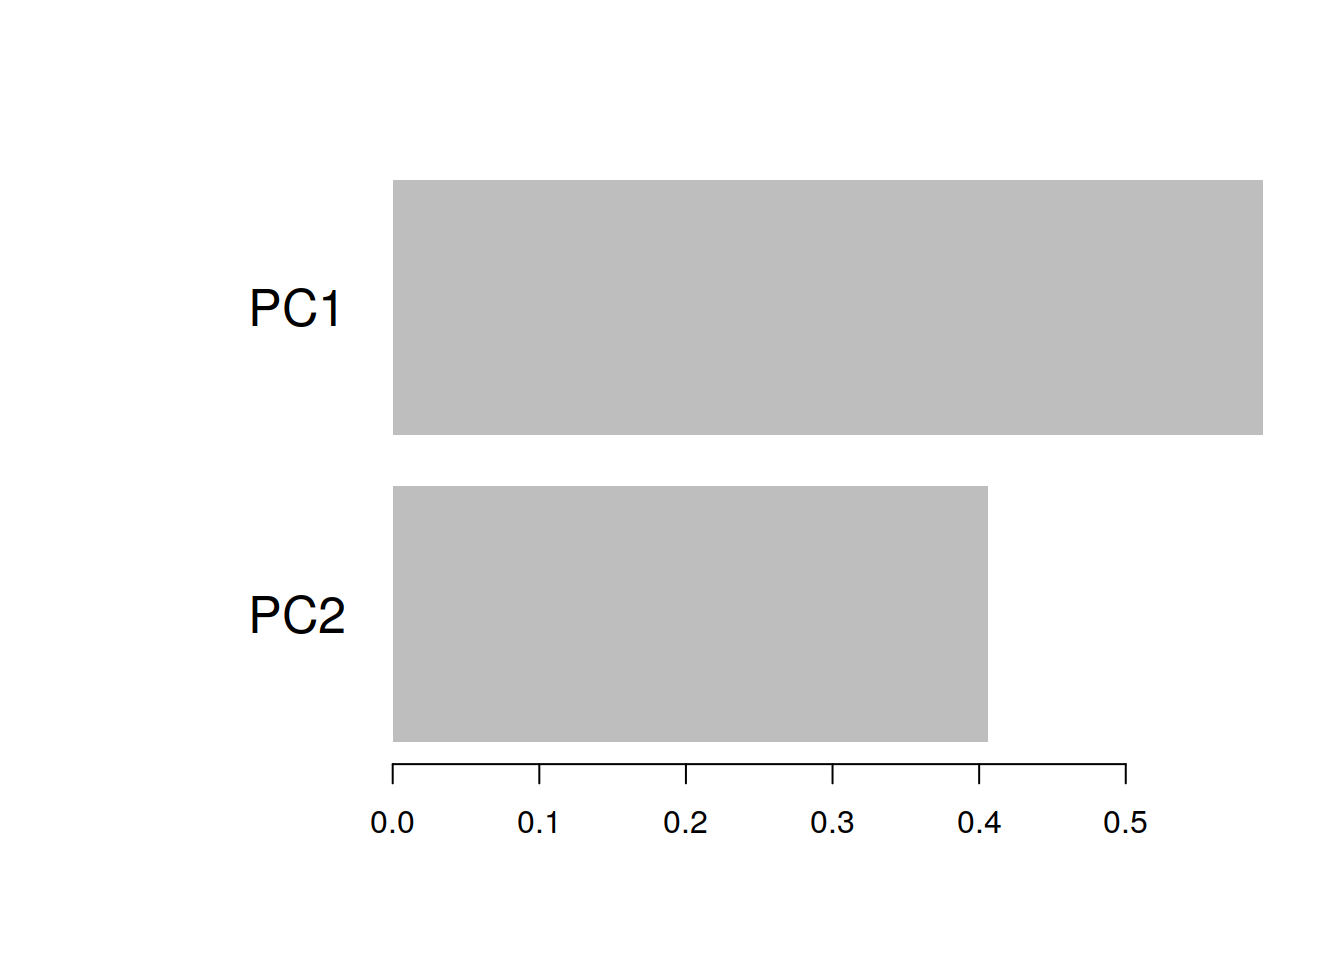
\includegraphics[width=1.0\textwidth]{xgb_coeff_pca}
        \caption{Modelo sobre el conjunto de datos al que aplicamos \textit{PCA}}
    \end{subfigure}
    \begin{subfigure}{0.45\textwidth}
        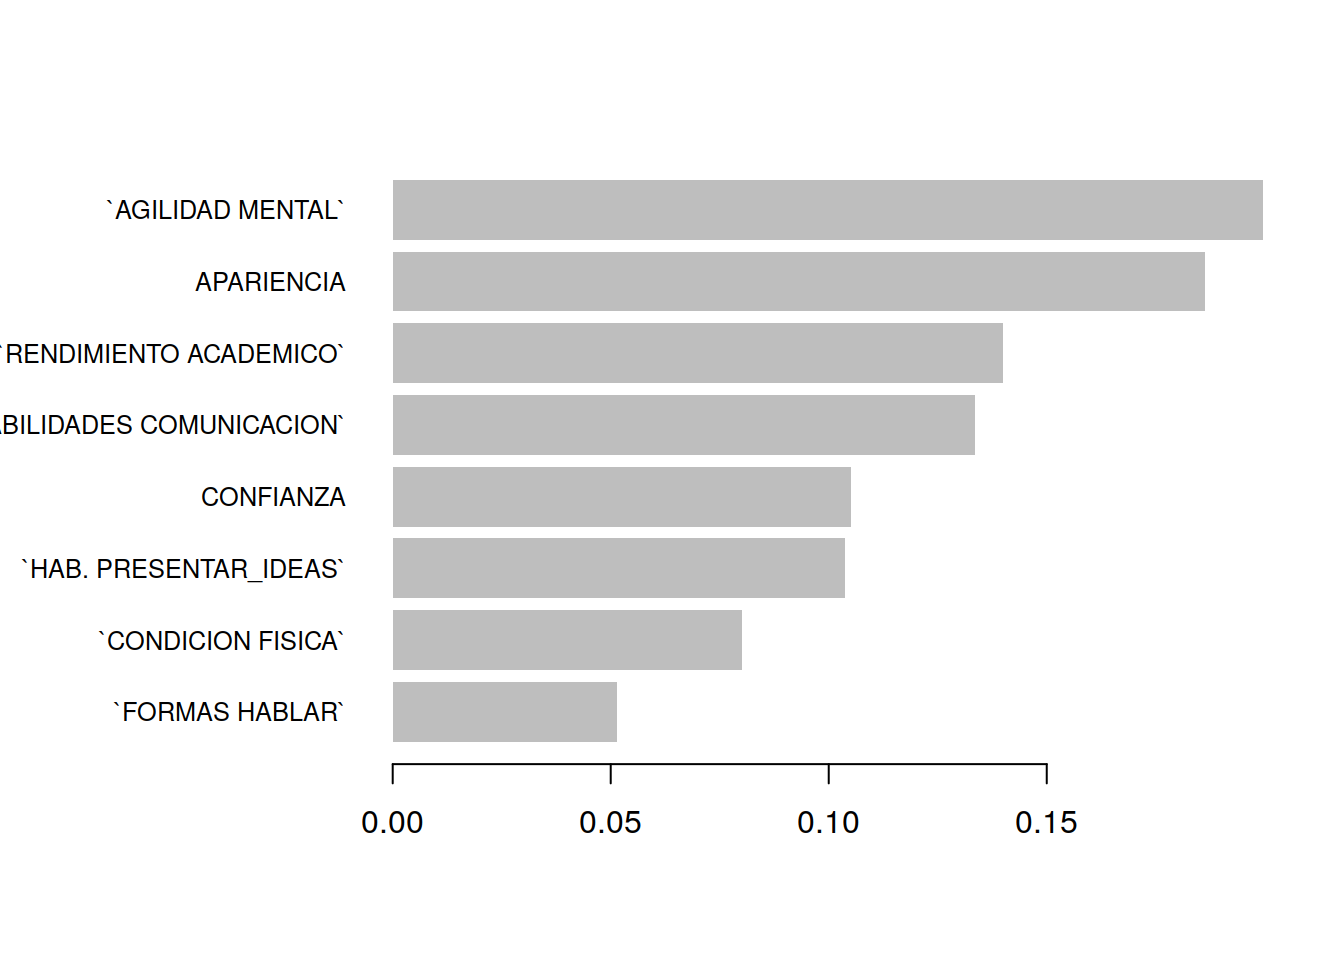
\includegraphics[width=1.0\textwidth]{xgb_coeff_orig}
        \caption{Modelo sobre el conjunto de datos original}
    \end{subfigure}

    \caption{Importancia de las variables a la hora de construir el modelo \textit{XGBOOST}}
\end{figure}

\subsection{Validación}

Empezamos mostrando el \textit{accuracy} de los modelos, tanto en entrenamiento como en \textit{test} \footnotemark:

\footnotetext{De esta forma, podemos diagnosticar ciertos problemas, principalmente, el \textit{overfitting}}

\begin{table}[H]
\centering
\begin{tabular}{|l|l|l|l}
\hline
    Modelo               & \textit{Train acc} & \textit{Test acc}          \\
\hline
Discriminante lineal     & 0.591178965224767  & 0.598319327731092 \\
Discriminante cuadrático & 0.706106870229008  & 0.697478991596639 \\
\textit{XGBOOST}         & 0.913910093299406  & 0.890756302521008 \\
\hline
\end{tabular}
\caption{\textit{Accuracy} de los tres modelos entrenados}
\end{table}

\subsection{Experimento adicional}

Como hemos visto que el mejor modelo es \textit{XGBOOST}, y como nos da algunas facilidades para interpretar los modelos obtenidos, usaremos este modelo. Además, usaremos el conjunto de datos original para simplificar el desarrollo del experimento. Esto porque, para aplicar \textit{PCA} o \textit{FA}, habría que aplicarlo a los dos conjuntos por separado, y ver si se obtienen mejores resultados que sin aplicar la transformación, usando \textit{k-fold Cross Validation}.

Realizamos la separación del conjunto de datos original en dos, uno conteniendo las variables que consideramos meritocráticas, y otro con las variables que consideramos no meritocráticas.

Como variables meritocráticas consideramos:

\begin{itemize}
    \item Rendimiento académico
    \item Agilidad mental
    \item Habilidad para presentar ideas
    \item Habilidades de comunicación
\end{itemize}

Como variables no meritocráticas consideramos:
\begin{itemize}
    \item Condición físicas
    \item Apariencia
    \item Formas de hablar
    \item Confianza
\end{itemize}

Realizamos un ajuste de hiperparámetros de los dos modelos \textit{XGBOOST}. Esto lo realizamos usando \textit{k-Fold Cross Validation} con \textit{Grid Search}. Los mejores parámetros para cada modelo son:

\begin{itemize}
    \item Modelo meritocrático: \lstinline{nrounds} = 480, \lstinline{max_depth} = 3, \lstinline{eta} = 0.3
    \item Modelo no meritocrático: \lstinline{nrounds} = 120, \lstinline{max_depth} = 5, \lstinline{eta} = 0.1
    \item Para el resto de parámetros, usamos el valor por defecto
\end{itemize}

Tras entrenar los modelos, los resultados obtenidos son:

\begin{table}[H]
\centering
\begin{tabular}{|l|l|l|l}
\hline
Conjunto de datos    & Train Acc         & Test Acc              \\
\hline
Meritocrático        & 0.733248515691264 & 0.694117647058824     \\
    \textbf{No meritocrático} & 0.719677692960136 & \textbf{0.715966386554622} \\
\hline

\end{tabular}
\caption{Resultados del experimento}
\end{table}

% TODO -- poner aqui las matrices de confusion

\newpage

\section{discusion} \label{section:Discusion}

TODO


% TODO -- Comentar, interpretar y explicar lo que significan los resultados

\newpage

\section{conclusion}

TODO

\newpage

\pagebreak


% Which style to use to show references
\bibliographystyle{ieeetr}

% Show the references
\bibliography{./References}

\end{document}
